
\section{Trees}
\label{sec:trees}

When we use a list for storing our data in a dynamic structure, we can
see there are two limitations: 

\begin{itemize}
\item Finding an element in the list takes a long time, proportional
  to the length of the list.
\item Keeping the elements of the list in order also takes a lot of
  time: you must find the place where the new element should be, and
  then insert it. 
\end{itemize}

Both seeking an element and inserting an element in a list require a
time that is proportional to the length of the list. They will take
(in average) twice as long in a list twice as big. 

We have seen that \emph{maps} provide a partial solution to the first
problem. By assigning a value with a key, they can access any element
immediately. However, maps have some problems too. Either you store
the keys on an array that you can access by index (i.e.~a hash of the
key) or you need a linked list of keys\ldots and then we are bumping
on the same problem again. 

Generally speaking, maps are used for relatively low numbers of
elements. When the number of elements is very big, and it 
is important to have them sorted, there is a better data structure:
the tree. 

A tree in computing is similar to a tree in nature because it has a
root and it has branches. Like a linked list, a tree is composed of
nodes/elements. Elements where branches start are usually called
\emph{nodes} and elements at the end of branches are usually
\emph{leaves}. In some trees you have data on nodes and leaves, while
in others you have data only on leaves. 

Trees are very important in computing. For example, the filesystem on
your hard disk, where you have stored all your files (including this
file you are reading now, your personal folders/directories, etc) has
a tree structure: folders are nodes and files are leaves.

Trees have a similar structure to lists, stacks, and queues; the main
difference is that each element points to two or more elements instead
of one. See 

\begin{figure}[hbtp]
  \centering
  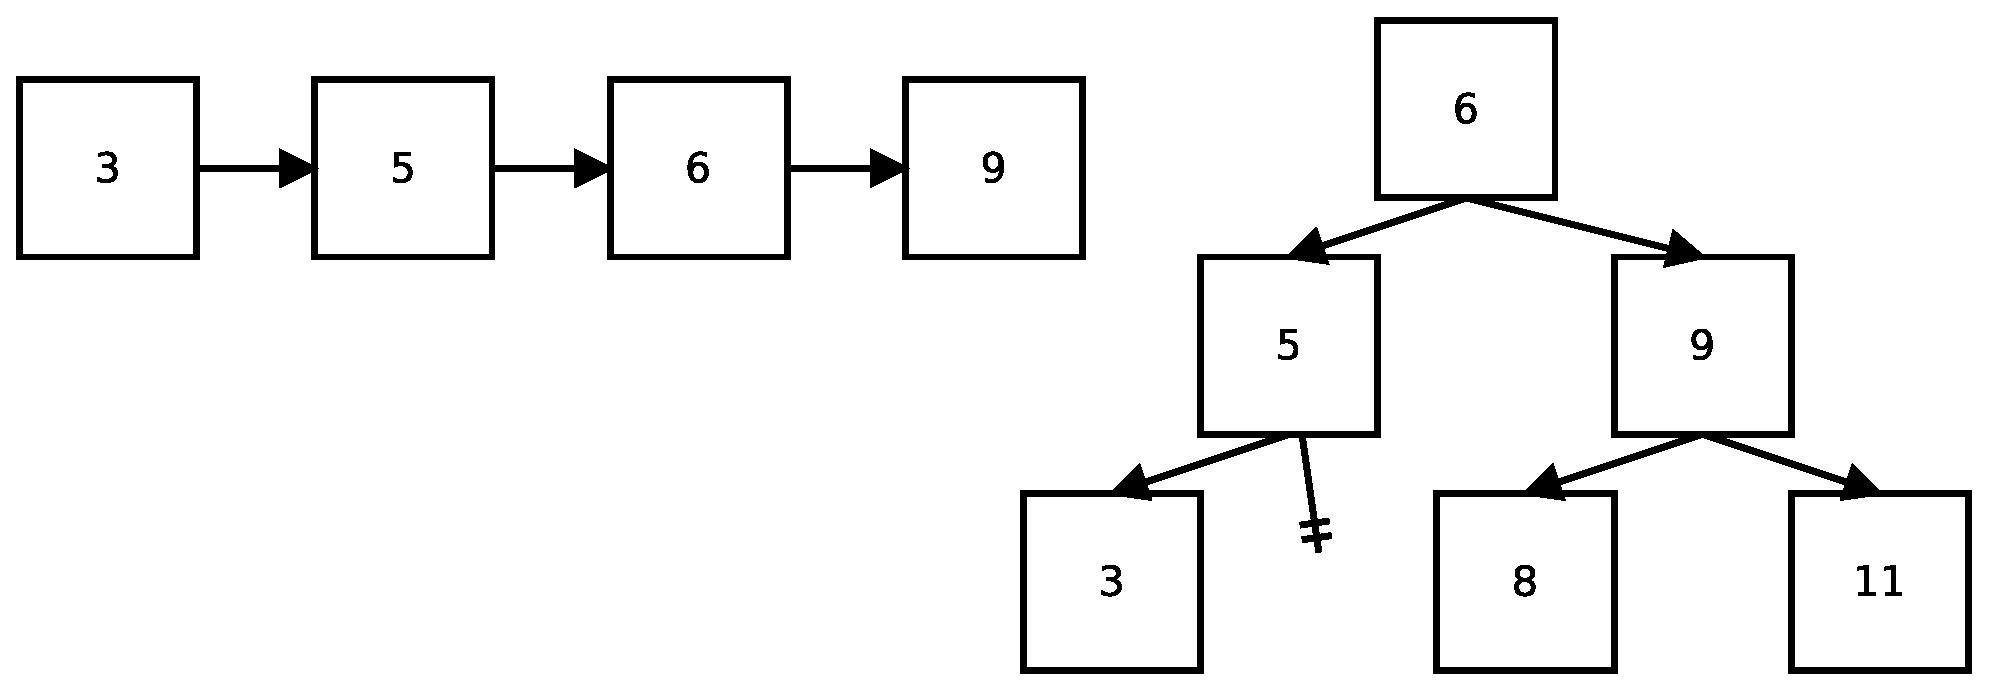
\includegraphics[width=\textwidth]{gfx/list-tree}
  \caption{In a singly-linked list, every element is connected to the next one. In a binary tree, every element is connected to two next elements.}
  \label{fig:listree}
\end{figure}

\begin{verbatim}
public class IntegerListNode {
    int value;
    IntegerListNode next;
    // ... methods would be here
}
(...)
public class IntegerTreeNode {
    int value;
    IntegerTreeNode left;
    IntegerTreeNode right;
    // ... methods would be here
}
\end{verbatim}

Trees where every node links to two other nodes are called
\emph{binary trees}. Binary trees are the most common types of
trees. But we can create trees of any cardinality:

\begin{verbatim}
public class IntegerTernaryTreeNode {
    int value;
    IntegerTernaryTreeNode left;
    IntegerTernaryTreeNode center;
    IntegerTernaryTreeNode right;
    // ... methods would be here
}
(...)
public class IntegerArbitraryTreeNode {
    int value;
    IntegerArbitraryTreeNode[] children;
    // ... methods would be here
}
\end{verbatim}

%%% Local Variables:
%%% mode: latex
%%% TeX-master: "main"
%%% End:
